\begin{figure}[htb]
 \begin{center}
   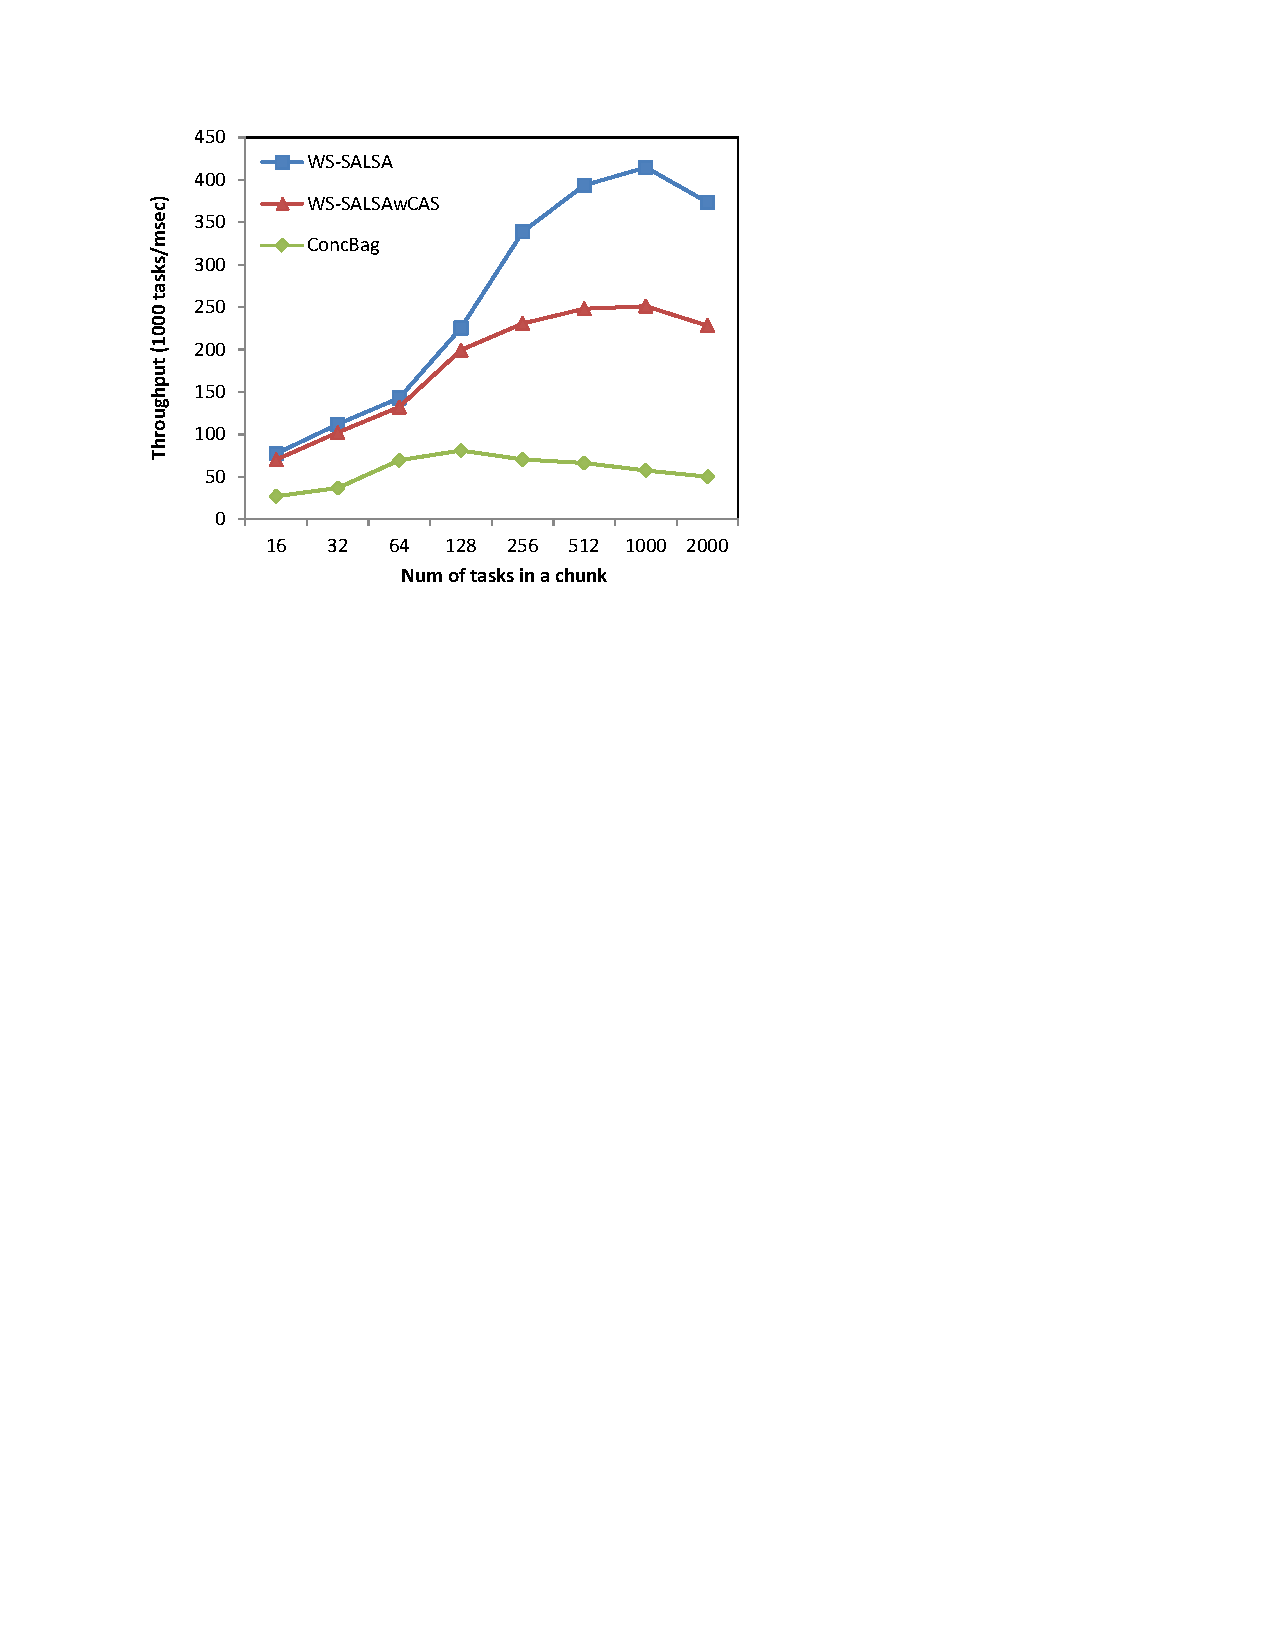
\includegraphics[width=0.45\textwidth]{figures/chunk-size}
 \end{center}
	\caption{\footnotesize{System throughput as a function of the chunk size. }}
	\label{fig:chunk-size}
\end{figure}
Figure~\ref{fig:chunk-size} shows the influence of the chunk size on system throughput for the chunk-based algorithms SALSA, SALSA+CAS and ConcBags in the $16/16$ workload. 
SALSA variations achieve their best throughput for large chunks with $1000$ tasks ($\sim8$KB size in $64$-bit architectures). The optimal chunk for ConcBags includes $128$ tasks. We believe that the reason that ConcBags cannot handle large chunk sizes is related to the fact that a consumer should linearly scan a chunk when seeking for a task to steal. In contrast, SALSA's algorithm of fast-path consumption keeps the index of the latest consumed task in the chunk node and therefore its consume operations terminate in $O(1)$ steps for every chunk size. 
In our evaluation we used optimal chunk sizes for each algorithm. 
